\begin{savequote}[45mm]
\ascii{Any fool can write code that a computer can understand. Good programmers write code that humans can understand.}
\qauthor{\ascii{- Martin Flower}}
\end{savequote}

\chapter{xUnit架构} 
\label{ch:xunit-architecture}

\begin{content}

本书通过使用\cpp{}设计和实现\ascii{xUnit}框架,透视极限编程在\cpp{}社区中的具体实践与运用,包括\ascii{简单设计},\ascii{TDD}、重构;也会深入体会正交设计、设计原则、设计模式、整洁代码、实现模式与习惯用法在编程实践中的具体运用;也会在面向对象、函数式、泛型编程不同编程范式之间切换自如;也会尝试\ascii{DSL}设计与实现,体会代码之美,设计之美,架构之美。

\end{content}

\section{xUnit家谱}

\begin{content}

\ascii{xUnit}表示一组单元测试框架集合,其基本架构思想起源于\ascii{SUnit}。\ascii{SUnit}由极限编程之父\ascii{Kent Beck}使用\ascii{SmallTalk}设计实现;随后,\ascii{Kent Beck}与\ascii{Erich Gamma}结对编程,移植实现了\ascii{Java}版本\ascii{JUnit}。

\ascii{JUnit}随着\ascii{Java}社区不断壮大,及其敏捷软件开发思潮的涌现,\ascii{JUnit}当前成为\ascii{Java}程序员最常使用的框架之一。目前,\ascii{JUnit}也在不对进化与演进,截止目前\ascii{JUnit5}也在完善与开发之中。

随之,各种编程语言社区都诞生了各种优秀的\ascii{xUnit}实现,包括基于\ascii{JVM}实现的高级编程语言系列。但是,它们都没有逃离\ascii{xUnit}基本框架和思维模式,唯有部分后起之秀在用户界面友好性方面取得极大的改进和提升。

一则,归功于编程语言的内在特性,因为有的编程语言天然地支持\ascii{DSL}的构建;二则,归功于同门竞争,例如,基于\cpp{}语言实现的\ascii{xUnit}在社区中就存在众多实现,而且在不断演进和革新。

\subsection{Google Test}

\ascii{Google Test}出自名家,自带光环。其功能强大,系统稳定,移植性良好,支持用例自动发现机制,相对于社区其他\ascii{xUnit}框架更显技高一筹,在\ascii{C++}社区占据主导地位。但是,\ascii{Google Test}也存在一些不尽人意的细节之处。

\begin{leftbar}
 \begin{c++}
#include <gtest/gtest.h>
#include <stack>

namespace {
  struct StackSpec : testing::Test {
  private:
    void SetUp() override {
      s.push(1);
      s.push(2);
    }

  protected:
    std::stack<int> s;
  };
}

TEST_F(StackSpec, apply_pop_0_time) {
  ASSERT_EQ(2, s.top());
}

TEST_F(StackSpec, apply_pop_1_time) {
  s.pop();
  ASSERT_EQ(1, s.top());
}

TEST_F(StackSpec, apply_pop_2_time) {
  s.pop();
  s.pop();
  ASSERT_TRUE(s.empty());
}
 \end{c++}
\end{leftbar}

\subsubsection{命名}

用例名字必须遵循标识符的严格命名格则,否则编译不能通过。一方面,新增/修改用例时,输入长串下划线极度枯燥乏味;另一方面,极大地降低了用例的可读性。

当用例命名成为程序员的一种负担,其质量将大大折扣。但是,测试用例是系统行为描述最重要的活“文档”,它与被测系统的代码一并入库,并保持同步。如果,测试用例命名质量不高,\ascii{"Test as Document"}的愿景只能沦为痴人说梦了。

\begin{leftbar}
 \begin{c++}
TEST_F(RobotCleanerTest, at_the_beginning_the_robot_should_be_in_at_the_initial_position) {
  ASSERT_EQ(Position(0, 0, NORTH), robot.getPosition());
}
 \end{c++}
\end{leftbar}

\subsubsection{重复}

\ascii{RobotCleanerTest}扮演\ascii{Fixure}的职责,但与每个\ascii{TEST\_F}分离实现,每个用例都要重复一次\ascii{RobotCleanerTest},程序员只能接受“拷贝-粘贴”,别无选择。

\begin{leftbar}
 \begin{c++}
struct RobotCleanerTest : testing::Test {
protected:
  RobotCleaner robot;
};
 
TEST_F(RobotCleanerTest, at_the_beginning_the_robot_should_be_in_at_the_initial_position) {
  ASSERT_EQ(Position(0, 0, NORTH), robot.getPosition());
}
 
TEST_F(RobotCleanerTest, should_be_face_west_after_turn_left) {
  robot.turnLeft();
  ASSERT_EQ(Position(0, 0, WEST), robot.getPosition());
}
  \end{c++}
\end{leftbar}

\subsubsection{隐晦}

\ascii{RobotCleanerTest}与\ascii{TEST\_F}分离实现,本应该被直观理解为类与成员函数之间的关系。理论上,\ascii{TEST\_F}能够直接获取到私有成员,例如\ascii{RobotCleanerTest::robot}。

不幸的是,\ascii{RobotCleanerTest}与\ascii{TEST\_F}存在隐晦的继承关系。如果用户不了解\ascii{Google Test}的实现机制,就根本无法理解成员变量\ascii{RobotCleanerTest::robot}为什么是\ascii{protected},而不是\ascii{private}。

\begin{leftbar}
 \begin{c++}
struct RobotCleanerTest : testing::Test {
private:  // should be protected
  RobotCleaner robot;
};
 
TEST_F(RobotCleanerTest, at_the_beginning_the_robot_should_be_in_at_the_initial_position) {
  ASSERT_EQ(Position(0, 0, NORTH), robot.getPosition());
}
  \end{c++}
\end{leftbar}

\subsubsection{误用}

用户也需要关注\ascii{TEST, TEST\_F}之间的区别,及其使用场景,无疑增加了用户的心智包袱。例如,用户在此处本应使用\ascii{TEST\_F},而误用为\ascii{TEST}。这个例子较为幸运,编译器提示\ascii{robot}变量未定义。但是,在特殊场景可能会逃出编译时检查,导致运行时用例失败。

\begin{leftbar}
 \begin{c++}
struct RobotCleanerTest : testing::Test {
protected:
  RobotCleaner robot;
};

// should be TEST\_F
TEST(RobotCleanerTest, at_the_beginning_the_robot_should_be_in_at_the_initial_position) {
  ASSERT_EQ(Position(0, 0, NORTH), robot.getPosition());
}
  \end{c++}
\end{leftbar}

\subsubsection{大小写}

覆写\ascii{Test::SetUp}时,经常将其错误地写为\ascii{setup, setUp, Setup},不经意地大小写错误导致运行时测试失败。当然,如果坚持使用\ascii{override}关键字提高编译时的安全性,可以将错误拦截至编译期。

\begin{leftbar}
 \begin{c++}
struct RobotCleanerTest : testing::Test {
private:
  // should be override
  virtual void Setup() {
    robot.reset();
  }
 
protected:
  RobotCleaner robot;
};
  \end{c++}
\end{leftbar}

\subsection{xUnit Mars}

假定预开发的系统名为\ascii{xUnit Mars},它完成类似\ascii{Google Test}的功能特性。相对于\ascii{Google Test},\ascii{xUnit Mars}定义了一套无歧义的\ascii{DSL},改善了用例描述的表达力,包括如下几个方面。

\begin{enum}
  \eitem{使用字符串描述用例,改善用例的表达力;}
  \eitem{在同一个类域内,使得TEST与SETUP/TEARDOWN关系更加紧密;}
  \eitem{避免setup/setUp/SetUp大小写混用而引发错误。}
\end{enum}

\begin{leftbar}
 \begin{c++}
#include <mars/mars.h>
#include <stack>

FIXTURE(StackSpec) {
  std::stack<int> v;   

  SETUP {
    v.push(1);
    v.push(2);
  }

  TEST("apply pop: 0 time") {
    ASSERT_EQ(2, v.top());
  }

  TEST("apply pop: 1 time") {
    v.pop();
    ASSERT_EQ(1, v.top());
  }

  TEST("apply pop: 2 times") {
    v.pop();
    v.pop();
    ASSERT_TRUE(v.empty());
  }
}; 
 \end{c++}
\end{leftbar}

\end{content}

\section{Mars架构}
	
\begin{content}

\subsection{初步架构}

\ascii{xUnit Mars}功能特性与\ascii{Google Test}存在明显的重合度。但是,\ascii{xUnit Mars}的用例设计风格与系统架构,相比\ascii{Google Test}存在巨大的差异。

在开发初期,\ascii{xUnit Mars}使用\ascii{Google Test}作为\ascii{TDD}的开发工具,待\ascii{xUnit Mars}完成基本功能,并发布稳定版本之后,可将既有测试用例重构为\ascii{xUnit Mars}风格。

基于\ascii{xUnit Mars}基本特性,可以改善使用\ascii{Modern C++}开发各类应用程序的用户体验。初步预想,\ascii{xUnit Mars}系统架构如\refig{mars-framework}所示。

\begin{figure}[H]
\centering
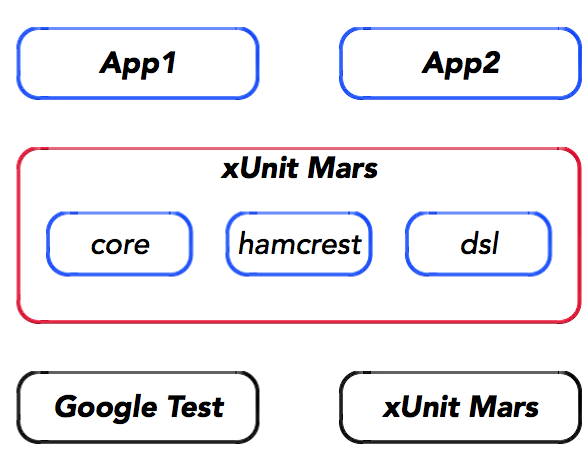
\includegraphics[width=0.5\textwidth]{figures/xunit/framework.png}
\caption{xUnit Mars: 系统架构}
 \label{fig:mars-framework}
\end{figure}

\end{content}
